\subsection{Two level system interacting with reservoir}

\begin{figure}[htbp]
    \centering
    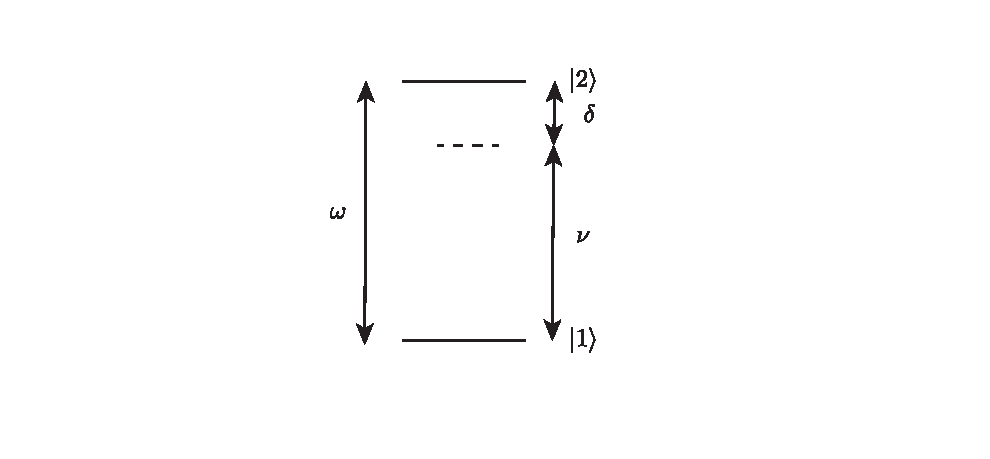
\includegraphics[width=\textwidth]{Chapter2_secs/twolevel.pdf}
    \caption{A two level system with energy difference $\omega$ in a light field with frequency $\nu$. $\delta = \nu - \omega$ is the detuning. }
    \label{fig:twolevel}
\end{figure}
A two level system shown in Fig.~(\ref{fig:twolevel}) interacts with light field via electric dipole interaction. 
\begin{equation}
    \hat{H} = -\Vec{d}\cdot \Vec{E}
\end{equation}
is the electric dipole interaction Hamiltonian where $\Vec{d} = e\Vec{r}$ is the dipole operator. The matrix element of dipole operator $\matrixel{L',m_L'}{\Vec{d}}{L,m_L}$ is nonzero only when $\Delta L = \pm 1$ and $\Delta m_L = 0$. The dipole operator doesn't interact with spin and nuclear angular momentum, so in the total angular momentum basis, the selection rule is 
\begin{equation}
    \Delta F = \pm 1.
\end{equation}
The Electric field
\begin{equation}
    \Vec{E} = E_x {\bf e_x} + E_y {\bf e_y} + E_z {\bf e_z}
\end{equation}
can be expressed in the basis of $\{ {\bf e_{\pm}},{\bf e_z}\}$,
\begin{equation}
    \Vec{E} = E_+ {\bf e_+} + E_- {\bf e_-} + E_z {\bf e_z}.
\end{equation}
Here,
\begin{equation}
    {\bf e_{\pm}} = \frac{{\bf e_x} \pm i{\bf e_y}}{\sqrt{2}}.
\end{equation}
The dipole interaction Hamiltonian is separated into the radial part and the angular part in the new basis,
\begin{equation}
    {\bf e_q}\cdot \Vec{r} = \sqrt{\frac{4\pi}{3}}\rho Y_{1,q}(\theta,\phi),
\end{equation}
here q = 1 for ${\bf e_+}$, q = -1 for ${\bf e_-}$ and q = 0 for ${\bf e_z}$, $Y_{1,q}(\theta,\phi)$ is the spherical harmonic function.

A two level system with energy difference $\omega$ interacts with electromagnetic field
\begin{equation}
    \Vec{E}(\Vec{r},t) = \Vec{E}_0 e^{-i(\nu t-\Vec{k}\cdot\Vec{r})} + \Vec{E}_0^*e^{i(\nu t-\Vec{k}\cdot\Vec{r})},
\end{equation}
the Hamiltonian is
\begin{equation}
    \hat{H} = \hbar \omega \dyad{2}{2} - (\Vec{\mu} \dyad{1}{2} + \Vec{\mu}^*\dyad{2}{1})\cdot\Vec{E}(\Vec{r},t).
\end{equation}
By transforming into a rotating frame, 
\begin{equation}
    \ket{\Tilde{2}} = e^{i\nu t}\ket{2},
\end{equation}
and neglecting the fast oscillating term $e^{\pm i\nu t}$, the Hamiltonian is transformed to
\begin{equation}
    \hat{H} = \hbar\delta \dyad{\Tilde{2}}{\Tilde{2}} + \hbar(\Omega \dyad{1}{\Tilde{2}} + \Omega^* \dyad{\Tilde{2}}{1}),
\end{equation}
Here,
\begin{equation}
    \Omega = \frac{\Vec{E}_0 \cdot \Vec{\mu}}{\hbar}.
\end{equation}
The frame transformation and the removal of the oscillating term is named after rotating wave approximation (RWA), it is widely used in atomic physics when atoms interact with near resonance high frequency optical field, and satisfying the condition $\delta \ll \nu, \omega$.

The Hamiltonian above describes a closed system, where the two level atom only interacts with the one single optical mode and the evolution of atomic states and photon states is coherent. In reality, the atom interacts not only with the optical field but also the vacuum modes in the environment. The vacuum modes are contiguous in free space and discrete in a cavity, the coupling between the atomic states to the vacuum modes leads to spontaneous emission of the excited state and causes incoherence. Wigner-Weisskopf theory \cite{scully1999quantum} represents the vacuum modes with quantized field operators and calculates spontaneous emission with Fermi's golden rule. The Hamiltonian of atomic system and vacuum modes is
\begin{equation}
    \hat{H} = \hbar \omega \dyad{2}{2} + \sum_j\hbar \nu (\hat{a}^\dag_j\hat{a}_j + \frac{1}{2}) - \sum_j(\hbar g_j \dyad{2}{1}\hat{a}_j + \hbar g_j^* \dyad{1}{2}\hat{a}^\dag_j),
\end{equation}
and $g_j$ is the coupling strength between the states $\ket{2,0}$ and $\ket{1,1_k}$. $\ket{1,1_k}$ is the state with one photon occupying mode $k$.
\begin{equation}
    \gamma = 2\pi \sum_j |g_j|^2\delta(\nu_j - \omega)
\end{equation}
is the result of spontaneous emission rate $\gamma$ and in free space
\begin{equation}
    \gamma = \frac{\omega^3|\mu|^2}{3\pi\epsilon_0\hbar c^3},
\end{equation}
which is also known as the Einstein A coefficient.

One way to describe both coherent and incoherent evolution is using density operator. The density operator is defined as
\begin{equation}
    \hat{\rho} = \sum_\alpha p_\alpha \dyad{\phi_\alpha}{\phi_\alpha}.
\end{equation}
Here, $\ket{\phi_\alpha}$ a quantum state and $p_\alpha$ is the probability that the state is in $\ket{\phi_\alpha}$. The states $\ket{\phi_\alpha}$ are not necessarily orthogonal to each other, but for the density operator representation to be valid, it has to satisfy the following condition,
\begin{equation}
    {\rm Tr}[\hat{\rho}] = 1.
\end{equation}
For any orthonormal basis $\{ \ket{n}\}$, 
\begin{equation}
    \sum_n \matrixel{n}{\hat{\rho}}{n} = 1,  and ~ {\rm Tr}[\hat{\rho}] = \sum_n \matrixel{n}{\hat{\rho}}{n},
\end{equation}
for the conservation of probability.

In the density operator representation, the expectation value of a dynamic variable $\hat{A}$ can be calculated using
\begin{equation}
    \expval{\hat{A}} = {\rm \hat{\rho}\hat{A}}.
\end{equation}

In the orthonormal basis $\{ \ket{n}\}$, the matrix element of the density operator is
\begin{equation}
    \rho_{n,n'} = \matrixel{n}{\hat{\rho}}{n'}.
\end{equation}
The diagonal elements $\rho_{n,n}$ represents the the probability that the state is in $\ket{n}$ and the off-diagonal elements $\rho_{n,n'}$ represents the expectation value of coherence between states $\ket{n}$ and $\ket{n'}$. If there exists a state $\ket{\phi}$ such that
\begin{equation}
    \hat{\rho} = \dyad{\phi}{\phi},
\end{equation}
the state represented by $\hat{\rho}$ is a pure state, otherwise, it is a mixed state. In quantum mechanics, the probability amplitude of states bear the full information, probability and coherence. The density operation representation loses the information of coherence of some states but the expectation value of coherence is preserved. 

For an open system, the physical system we are interested in interacts with the environment, or sometimes called reservoir. The reservoir can contain a large number of degrees of freedom, for example, vacuum modes and other electromagnetic fields modes. The large number of degrees of freedom of the reservoir makes it hard to study its dynamics, however, in many cases, we are not actually interested in learning about the evolution of the reservoir. In these cases, it is useful to ignore the dynamics of the reservoir and only keep the effect the reservoir has on the system. By making this assumption, the coherent evolution of the system and the reservoir is lost and there exists decoherence in the dynamic of the system, so density operator is widely used to describe the open system.

The full Hamiltonian is
\begin{equation}
    \hat{H} = \hat{H}_S +\hat{H}_R + \hat{H}_{SR} 
\end{equation}
and under Heisenberg's equation, the evolution of the density operator is
\begin{equation}
    \frac{d}{dt}\hat{\rho} = \frac{1}{i\hbar}\left[ \hat{H},\hat{\rho} \right]
\end{equation}
Assume the interaction operator takes the form
\begin{equation}
    \hat{H}_{SR}  = \hat{S}\hat{R}^\dag + \hat{S}^\dag\hat{R}.
\end{equation}
To ignore the dynamics of the reservoir and only keep the effects it has on the system, we need to make two assumptions. First, factorize the reservoir operator
\begin{equation}
    \hat{R} \approx f(t)\hat{\Tilde{R}}.
\end{equation}
The function $f(t)$ characterizes the time evolution of the reservoir, and it is often assumed that the reservoir is stationary in the stochastic process language. The auto-correlation function of $f(t)$ is defined as
\begin{equation}
    ACF_f(t-t') = \expval{(f(t)-\expval{f(t)})(f(t')-\expval{f(t')})}.
\end{equation}
The correlation time $t_c$ of the function $f(t)$ is defined as the width of the peak of $ACF_f(t-t')$. 
The first assumption of reservoir is that $t_c \ll 1$, which means the reservoir has Markovian property, it quickly forgets about its previous state does not keep the memory of interacting with the system.

The second assumption is the reservoir is large enough that the system can hardly affect its state. Again, this means that the reservoir is stationary. Under these assumptions, the dynamics of the system is derived and expressed in terms of the reduced density operator
\begin{equation}
    \hat{\rho}_S = {\rm Tr}_{\rm R} [\hat{\rho}],
\end{equation}
which takes the average of the reservoir state by tracing out the reservoir degrees of freedom.

For a two level system
\begin{equation}
    \hat{H}_S = \hbar\delta \dyad{2}{2} + \hbar(\Omega \dyad{1}{2} + \Omega^* \dyad{2}{1}),
\end{equation}
the density operator evolves under eqaution
\begin{align}\label{OBE}
    &\dot{\rho}_{22} = -\gamma(\overline{n} + 1)\rho_{22} + \gamma\overline{n}\rho_{11} + i\Omega^*\rho_{21} - i\Omega\rho_{12}\\\nonumber
    &\dot{\rho}_{11} = \gamma(\overline{n} + 1)\rho_{22} - \gamma\overline{n}\rho_{11} - i\Omega^*\rho_{21} + i\Omega\rho_{12}\\\nonumber
    &\dot{\rho}_{12} = -\frac{\gamma}{2}(2\overline{n} + 1)\rho_{12} - i\delta\rho_{12} - i\Omega^*(\rho_{22}-\rho_{11})\\\nonumber
    &\dot{\rho}_{21} = -\frac{\gamma}{2}(2\overline{n} + 1)\rho_{21} + i\delta\rho_{21} + i\Omega(\rho_{22}-\rho_{11})\\\nonumber
\end{align}
This is known as the {\bf Optical Bloch equations}, and also called \textbf{Master equation} \cite{metcalf2007laser}. The first two equations describe the evolution of the probability of occupying the states $\ket{2}$ and $\ket{1}$.  The third and fourth equations describe the evolution of expected coherence between states $\ket{1}$ and $\ket{2}$. The term $\gamma(\overline{n} + 1)\rho_{22}$ combines spontaneous emission ($\gamma\rho_{22}$) and stimulated emission ($\gamma\overline{n}\rho_{22}$). 

